\section{Effective Moisture Penetration Depth (EMPD) Model}\label{effective-moisture-penetration-depth-empd-model}

\subsection{Overview}\label{overview-014}

Moisture has little effect on heating system performance, but a profound effect on the performance of air conditioning systems.~ In order to accurately describe building performance during periods when cooling is needed, it is very important to know the moisture conditions of the building.~ If one assumes that all building moisture is contained in the room air, then one ignores the fact that the materials that bound the room (e.g.~wall surfaces, furnishings, linens, etc.) store and release moisture.~ Thus, to assume that the only moisture that effects cooling system performance is contained in the room air is a false, and it can lead to significant error in the prediction of room moisture conditions and cooling system loads.

The EMPD (Effective Moisture Penetration Depth) model is a simplified, lumped approach to simulate surface moisture adsorption and desorption.

\subsection{EMPD Model Description}\label{empd-model-description}

The EMPD concept assumes that a thin layer ($\delta$\(_{M}\)) close to the wall surface behaves dynamically and exchanges moisture with the air domain when exposed to cyclic air moisture pulses.~ For short periods where the cyclic integral of the total moisture adsorption and desorption is near zero (i.e.~there is no net moisture storage), the EMPD concept has been shown to be a reasonable approximation of reality (Kerestecioglu et al, 1989).~ In other words, the following constraint must be met:

\begin{equation}
\int_{{\tau_1}}^{{\tau_2}} {\frac{{dU}}{{d\tau }}} d\tau  = 0
\end{equation}

where, $\tau$\(_{2}\)-$\tau$\(_{1}\) denotes the finite time interval over which the equation holds.~ The EMPD model assumes no spatial distribution of moisture content across the thickness (L) of the solid; rather, a thin layer ($\delta$\(_{M}\)) of uniform moisture content (U) is assumed to represent the total moisture content of the solid. This may be mathematically stated as:

\begin{equation}
\int_0^L {U(x)dx = U{\delta_M}}
\end{equation}

For most building materials, the equilibrium moisture sorption isotherm can be defined by the following general equation (Kerestecioglu et al. 1988):

\begin{equation}
U = a{\varphi ^b} + c{\varphi ^d}
\end{equation}

where

\begin{equation}
\varphi  \approx \frac{{{W^*}}}{{{W_{sat}}^*}}
\end{equation}

and

\begin{equation}
{W_{sat}}^* = \frac{1}{{{R_v}{\rho_a}{T^*}}}\exp \left( {23.7093 - \frac{{4111}}{{{T^*} - 35.45}}} \right)
\end{equation}

~Given that U = U(W\(^{*}\),T\(^{*}\)), the moisture content may be differentiated with respect to time in the following manner:

\begin{equation}
\frac{{du}}{{d\tau }} = \frac{{\partial U}}{{\partial {W^*}}}\frac{{d{W^*}}}{{d\tau }} + \frac{{\partial U}}{{\partial {T^*}}}\frac{{d{T^*}}}{{d\tau }} = {A_T}\frac{{d{W^*}}}{{d\tau }} - {B_\rho }\frac{{d{T^*}}}{{d\tau }}
\end{equation}

where A\(_{T}\) and B\(_{\rho}\) are the isothermal moisture capacity and thermo-gradient coefficient, respectively.~ From Eqs. , and , they can be expressed as:

\begin{equation}
{A_T} = \frac{{ab{\varphi ^b} + cd{\varphi ^d}}}{{{W^*}}}
\end{equation}

and

\begin{equation}
{B_\rho } =  - \left[ {\frac{1}{{{T^*}}} - \frac{{4111}}{{{{({T^*} - 35.45)}^2}}}} \right]*(ab{\varphi ^b} + cd{\varphi ^d})
\end{equation}

The lumped mass transfer equation for the i-th solid domain may be written as

\begin{equation}
{(A{\rho_b}{\delta_M})_i}\frac{{d{U_i}}}{{d\tau }} = {h_{M,i}}{A_i}({W_r} - {W_i}^*)
\end{equation}

Using Eqs. , , and , one obtains the final equation needed for closure moisture transfer at internal surface.

\begin{equation}
{({A_i}{\rho_b}{\delta_M}{A_T})_i}\frac{{d{W_i}^*}}{{d\tau }} = {h_{M,i}}{A_i}({W_r} - {W_i}^*) + {(A{\rho_b}{\delta_M}{B_\rho })_i}\frac{{d{T_i}^*}}{{d\tau }}
\end{equation}

The energy equation for the envelope contains the surface temperature and is given by the conduction equation

\begin{equation}
\rho {C_p}\frac{{dT}}{{d\tau }} = \nabla  \cdot (k\nabla T)
\end{equation}

with the boundary conditions at interior surface

\begin{equation}
- k\nabla T =  - {q_T}'' + {h_T}({T^*} - {T_r}) + \lambda {h_M}({W^*} - {W_r})
\end{equation}

A more detailed account of the numerical solution procedure can be found in Kerestecioglu et al. (1988).

\subsection{EMPD Value Determination}\label{empd-value-determination}

An effective moisture penetration depth may be determined from either experimental or detailed simulation data by using actual surface areas and moisture vapor diffusivity.~ An empirical function derived from the detailed simulation may be used to determine the EMPD value (Kerestecioglu et al, 1989):

\begin{equation}
{\delta_M} = 12.567024 - 12.21373*\exp \left( { - 267.0211*{D_v}^{0.7}*{\xi ^{ - 0.7}}} \right)
\end{equation}

where

\begin{equation}
\xi  = \left| {\frac{{\Delta \varphi }}{{\Delta \tau }}} \right|
\end{equation}

Figure~\ref{fig:limit-of-effective-penetration-depth-values} gives the EMPD values to be used for various vapor diffusivities evaluated at different ambient excitations.

\begin{figure}[hbtp] % fig 17
\centering
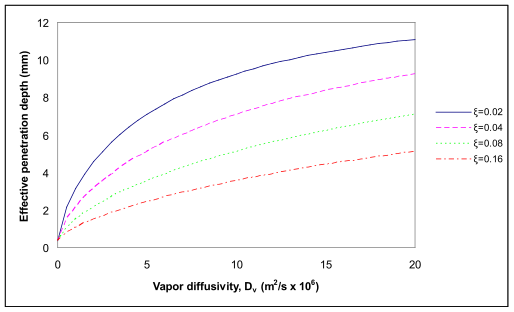
\includegraphics[width=0.9\textwidth, height=0.9\textheight, keepaspectratio=true]{media/image241.svg.png}
\caption{Limit of Effective Penetration Depth Values for Various Vapor Diffusivities at Different Ambient Excitations. \protect \label{fig:limit-of-effective-penetration-depth-values}}
\end{figure}

\subsection{EMPD Nomenclature}\label{empd-nomenclature}
\begin{align*}  
  A  &= \text{Area} [m^{2}] \\
  A_{T}  &= \text{Isothermal moisture capacity} [m/(^{3}/kg] \\
  B_{\rho}  &= \text{Thermo-gradient coefficient} [kg/kg-K] \\
  C_{p}  &= \text{Specific heat} [J/kg-K] \\
  h_{M}  &= \text{Convective mass transfer coeff.} [kg/m^{2}-s] \\
  h_{T}  &= \text{Convective heat transfer coeff.} [W/m^{2}-K] \\
  k  &= \text{Thermal conductivity} [W/m-K] \\
  L  &= \text{Length} [m] \\
  q''_{T}  &= \text{Imposed heat flux} [W/m^{2}] \\
  R_{v}  &= \text{Ideal gas constant} [461.52 J/kg-K] \\
  T  &= \text{Temperature} [K] \\
  U  &= \text{Moisture content} [kg/kg] \\
  W  &= \text{Humidity ratio} [kg/kg]
\end{align*}

\subsubsection{Greek letters}\label{greek-letters}
\begin{align*}  
  \delta\PB{M}  &= \text{Effective penetration depth for moisture equation} \bracketunits{\meter} \\
  \lambda       &= \text{Heat of vaporization} \bracketunits{\joule\per\kilogram} \\
  \rho          &= \text{Density} \bracketunits{\kilogram\per\cubic\meter} \\
  \tau          &= \text{Time} \bracketunits{\second} \\
  \varphi       &= \text{Relative humidity - fraction, 0 to 1} \bracketunits{-} \\
  \xi           &= \text{Ambient moisture excitation rate} \bracketunits{\per\hour}
\end{align*}

\subsubsection{Subscripts and superscripts}\label{subscripts-and-superscripts}
\begin{align*}  
  a             &= \text{Air} \\
  b             &= \text{Bulk} \\
  *             &= \text{Surface} \\
  i             &= \text{i-th surface} \\
\end{align*}

\subsection{References}\label{references-019}

Kerestecioglu, A., Swami, M., Dabir, R., Razzaq, N., and Fairey, P., 1988, ``Theoretical and Computational Investigation of Algorithms for Simultaneous Heat and Moisture Transport in Buildings,'' FSEC-CR-191-88, Florida Solar Energy Center, Cape Canaveral, FL.

Kerestecioglu, A., M. Swami and A. Kamel, 1989, ``Theoretical and Computational Investigation of Simultaneous Heat and Moisture Transfer in Buildings: Effective Penetration Depth Theory.''~ ASHRAE Winter Meeting, Atlanta, GA.

Kerestecioglu, A., M. V. Swami, P. Brahma, L. Gu, P. Fairey, and S. Chandra, 1989, ``FSEC 1.1 User's Manual,'' Florida Solar Energy Center, Cape Canaveral, FL
